\section{Echtzeitholographie}
\subsection{Versuchsbeschreibung}
Bei der Echtzeitholographie wird ein Hologramm aufgenommen und dieses mit dem Bild des Objektes überlagert. Unterschiede zwischen dem Objekt und seinem Hologramm können dann als Interferenzmuster beobachtet werden, solange sie nicht zu groß sind. In unserem Experiment wollen wir mit dieser Methode die resonanten Schwingungen einer fest eingespannten Aluminiumplatte untersuchen. Dazu nehmen wir zuerst ein Hologramm von dieser auf und entwickeln dieses. Mit einem Lautsprecher und einem Frequenzgenerator wird dann die Platte in Schwingung versetzt. Das Interferenzmuster erlaubt dann Rückschlüsse auf die Verformung und zeigt bei den Resonanzfrequenzen ein charakteristisches Muster.

\subsection{Durchführung und Auswertung}

Wir haben den Aufbau analog wie im vorherigen Versuchsteil verwendet. Anstelle der Stäbe haben wir allerdings die Aluminiumplatte eingebaut und den Lautsprecher hinter dieser plaziert. Da das Interferenzmuster Änderungen im Wellenlängenbereich anzeigt, sollte die Photoplatte nicht bewegt werden. Die Aufnahme und Entwicklung findet daher "`in-situ"' statt, d.h. in einem Tauchbecken am Ort der Aufnahme. 

 
\begin{figure}[ht]
 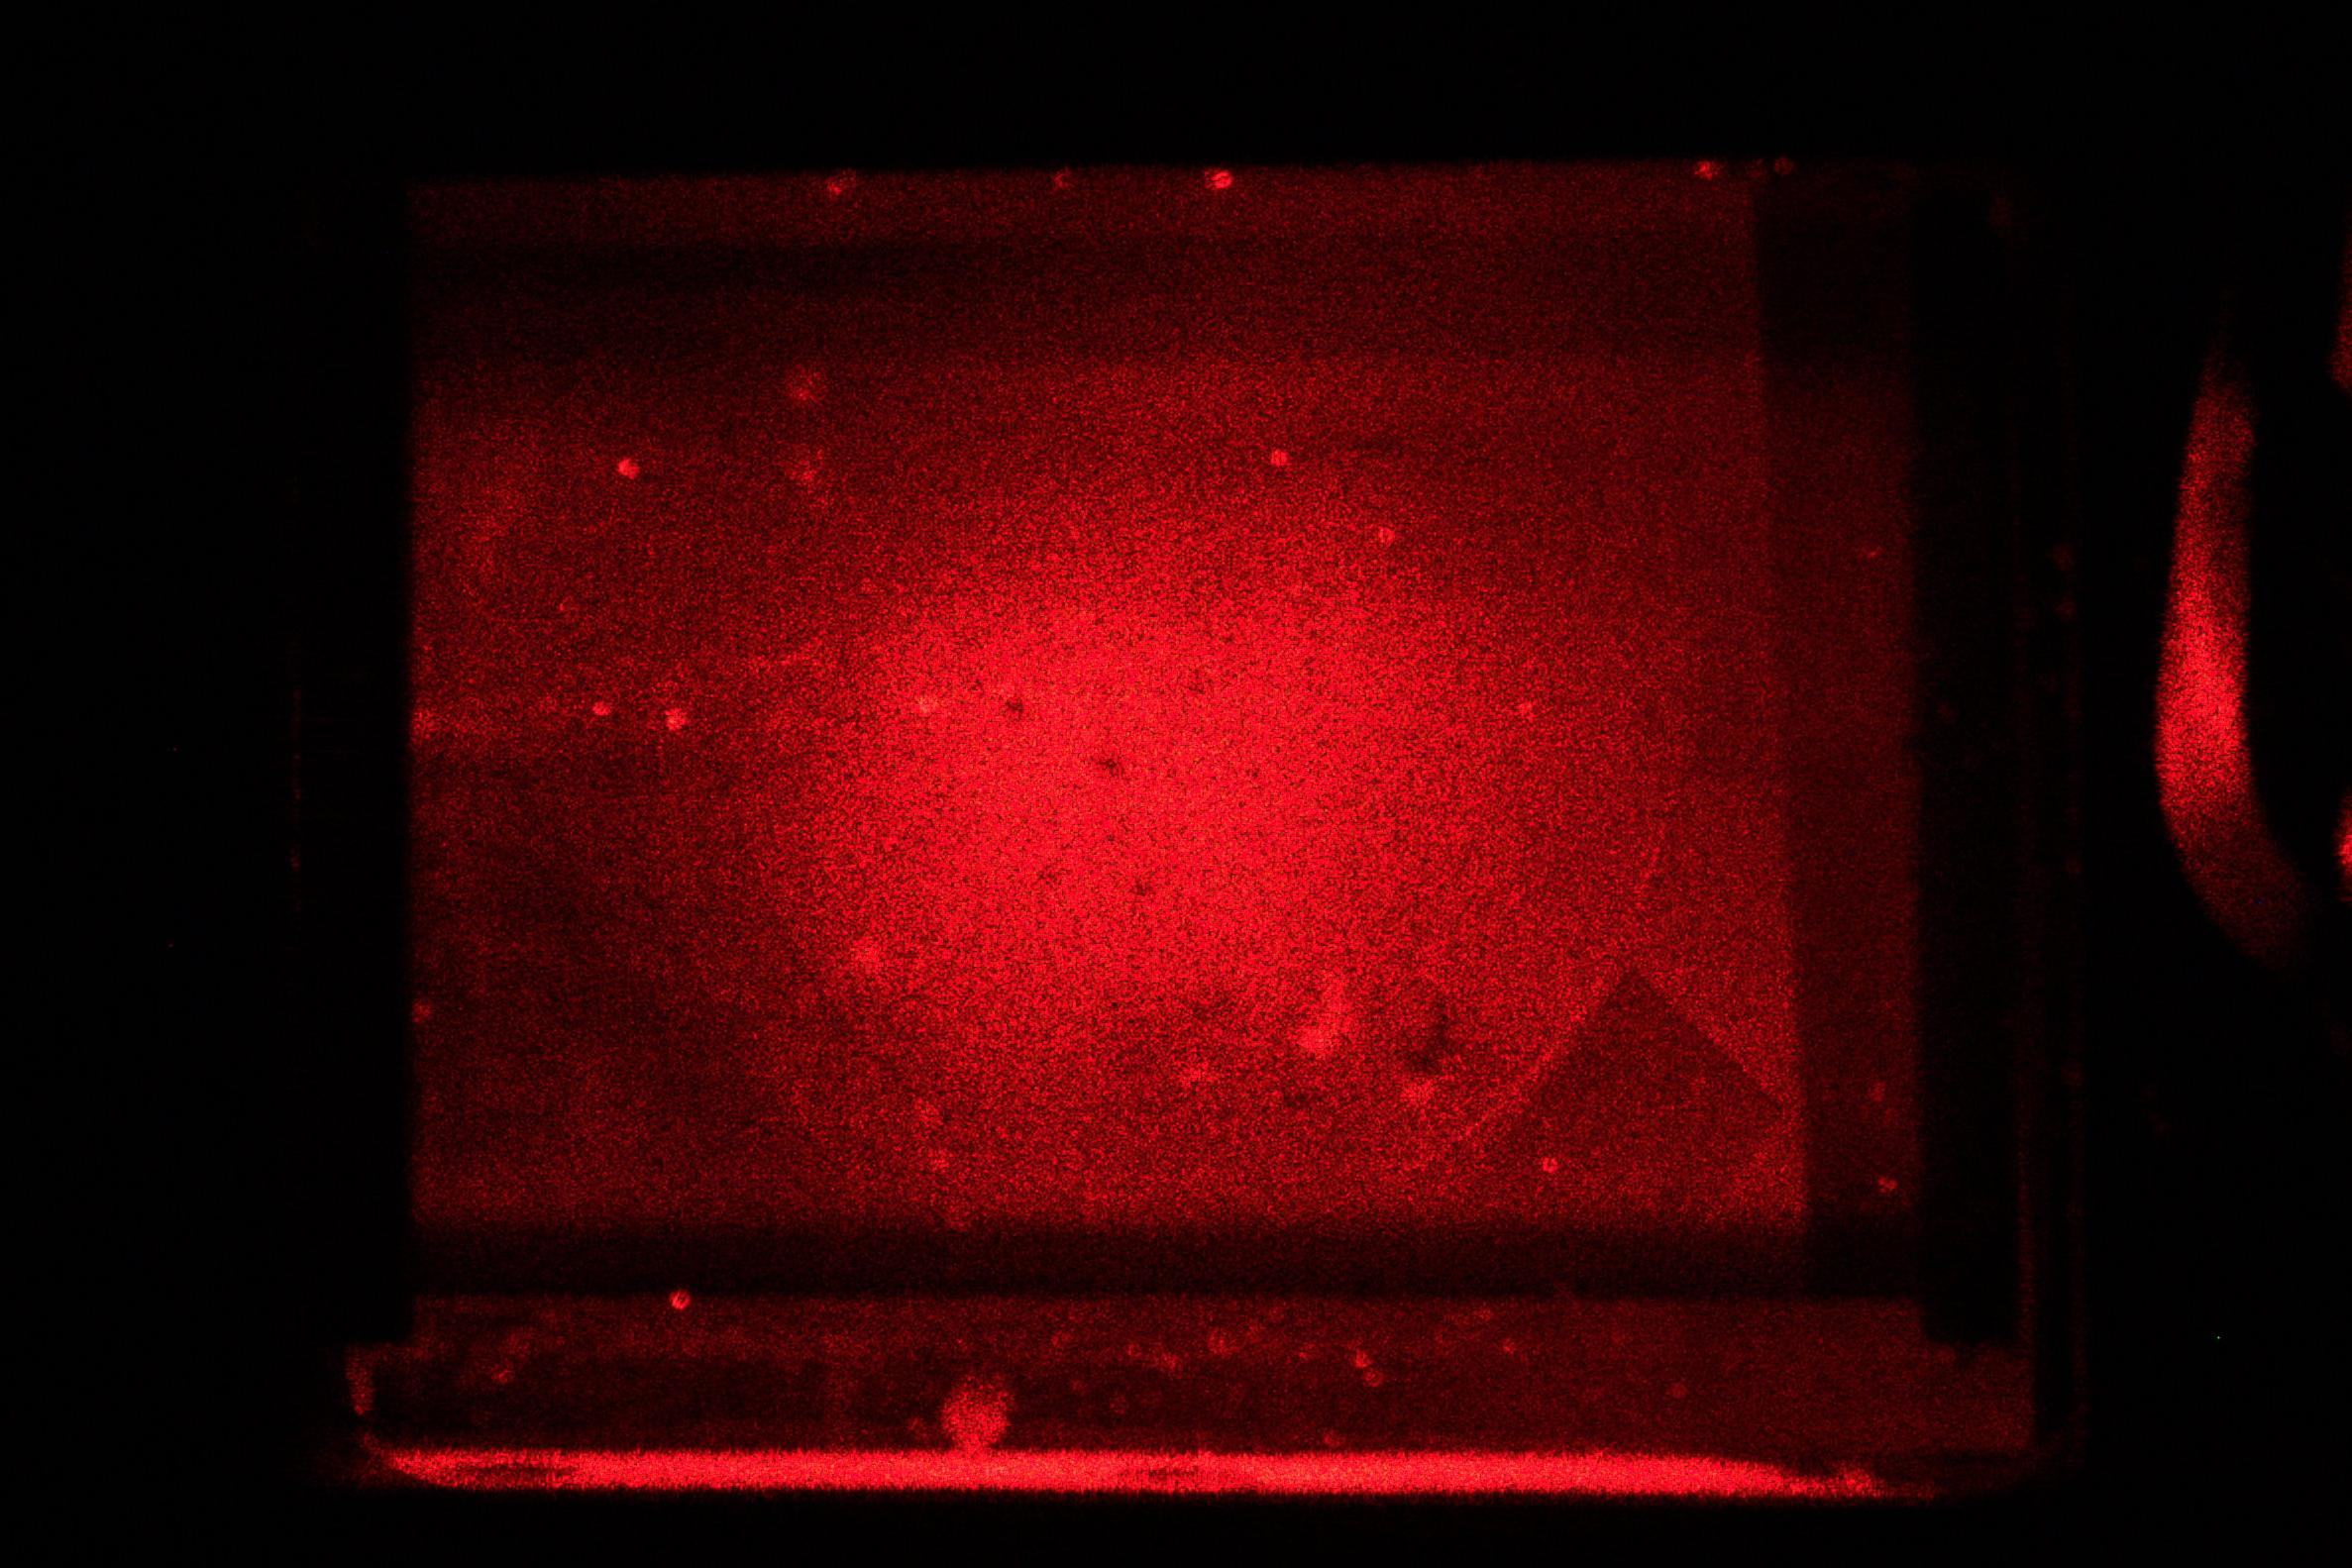
\includegraphics[width=\textwidth]{Photos/IMG_3927.jpg}
 \caption{Hologramm der Aluminiumplatte}
\end{figure}

